\chapter{Introduction}
\label{ch:intro}

\todo{Maybe reorg: Motivation to go into Background instead?}

\section{Motivation}

Developing software is difficult. Developing software that is bug-free is all but impossible. Programming languages like C and C++ (the so-called "low-level" programming languages~\footnote{"low-level" is traditionally used to indicate that the level of abstraction used by these  programming languages is relatively close to that of the hardware}) offer a great deal of control to the programmer, allowing them to write small and efficient computer programs. However, they also require the programmer to take a great deal of care with their development: the same level of control that allows extremely efficient software to be built also places a large burden on the developer, as making mistakes has steeper consequences than in high-level, safer programming languages (such as Java or C\#).

Typically, low-level programming languages require the programmers to manage memory manually, while higher-level languages generally include a garbage collector (GC) that frees the programmer from this burden. Managing memory manually means that objects whose lifetime is dynamic (not tied to a particular program scope) have to be \emph{allocated} as well as \emph{deallocated} (freed) explicitly.

In C, such memory allocation typically occurs using the \lstinline!malloc()! or \lstinline!calloc()! functions. These allocate a region inside the \emph{heap memory} of the application, reserving it for use, and returning a pointer (typically, an untyped \lstinline!void *!) to it. On the x86 and x86-64 architectures, which we will mainly concern ourselves with in this thesis, a pointer is just a linear memory address: a number representing the index of the first byte of the pointed region in the main memory. This makes pointer arithmetic, such as accessing \lstinline!numbers[4]! in a \lstinline!int *numbers! very easy and efficient to perform: just load \lstinline!sizeof(int)! bytes from the memory address \lstinline!(uintptr_t)numbers + 4 * sizeof(int)!. Conversely, after we are done with using a given memory region, we can and should deallocate it using the \lstinline!free()! function. This marks the memory region as no longer in use, and potentially reusable -- a characteristic that forms the basis of this thesis.

In C++, memory allocation typically happens using the \lstinline!new! or \lstinline!new[]! operators, and deallocation using the \lstinline!delete! or \lstinline!delete[]! operators. However, these behave exactly like C's \lstinline!malloc()! and \lstinline!free()! in all ways that are important from a memory management point of view. I should note that in modern C++, the use of such memory management is discouraged and generally unnecessary since \emph{smart pointers} -- wrappers around pointers that automate the lifecycle management of the pointed memory region, conceptually similarly to a garbage collector -- were introduced. However, a lot of applications are still being developed and maintained that do not make use of such features.

Making mistakes with manual memory management is very easy. Allocating but not freeing a memory region even after it's no longer used is called a \emph{memory leak} and it increases the memory usage of the application, often in an unbounded manner, potentially until a crash occurs due to insufficient memory. Attempting to deallocate an object twice -- \emph{double free} -- causes the memory allocator to attempt to access accounting data stored typically alongside the user data in the since-freed region, often leading to seemingly nonsensical behaviour or a crash, given that the region may have been re-used. Accessing an offset that falls outside the memory region reserved for the object -- \emph{out-of-bounds access}, sometimes also called \emph{buffer overflow} or \emph{buffer underflow} -- can lead to reading unexpected data or overwriting an unrelated object, again often causing hard-to-understand bugs and crashes. One example for this would be attempting to write to \lstinline!numbers[5]! when only enough space to hold 5 elements was allocated, e.g. using \lstinline!int *numbers  = malloc(5 * sizeof(int))! (recall that in C and related languages, indexes start at 0, so the first item is located at index 0, the second at index 1, and so on). Finally, accessing a memory region that has been deallocated -- \emph{use after free} -- is similarly problematic. This generally occurs when a pointer is not cleaned up along with the object it referenced, leaving it dangling; often also called a \emph{dangling pointer}.

Besides the instability and general mayhem that such memory errors routinely cause, they can also leave the application vulnerable to attacks, for instance by enabling unchecked reads or writes to sensitive data, sometimes even allowing an attacker to hijack the control flow of the application, execute almost arbitrary instructions, and in essence take over the application.

It should be clear by now why modern, "high-level" programming languages restrict or completely prohibit the direct use of pointers, often by making it impossible and unnecessary to manage memory manually. In such languages, the programmer can perform allocations only by creating objects (preventing another class of bugs relating to the use of uninitialized memory), and leaving their deallocation to the runtime environment, commonly its component called the garbage collector (GC). The GC will periodically analyse the memory of the application, and upon finding objects that are no longer referenced, marks them for reclaiming, and eventually deallocating them automatically. This, of course, comes at a cost in performance, often one that's unpredictable as the GC is controlled by the runtime environment as opposed to the user code. (It's worth  noting that this scheme doesn't protect against all possibilities of memory errors; for instance, leaks are still both possible and common.)

A notable exception is the Rust programming language, which, while does allow pointers, heavily restricts how they can be used, preventing any code that could potentially be unsafe. It does so using static (compile-time) checking using their so-called \emph{borrow checker}. However, realizing that in doing so it also disallows some valid uses of pointers, it also provides an escape hatch, allowing code sections to be marked as \emph{unsafe} and go unchecked. (For example, it's not possible to implement a linked list in safe Rust, and even the built-in \lstinline!vec! type is written using unsafe code.) Another programming language that follows a similar pattern is C\#: normally used as a high-level, managed language employing a GC, it also allows pointers to be used directly in code marked as unsafe~\footnote{Usage of raw pointers in an otherwise managed environment comes with caveats; for instance, the memory is often compacted after GC passes with the surviving objects moved next to each other to reduce fragmentation. Such relocation is not possible if there are raw pointers in play; therefore, programmers are required to mark the pointers they use as \emph{pinned} using the \lstinline!fixed()! construct.}.

Still, applications written in languages like C or (older) C++ with no safe alternatives to pointers have been written and are being maintained, and these applications remain affected by memory errors. Significant amount of research has been and continues to be conducted in this topic, as such applications are often high-value targets for attackers: operating system kernels, device drivers, web servers, anti-virus programs are commonly developed using these technologies.

This thesis is focused specifically on dangling pointer errors, a class of memory issues defending against which has traditionally been difficult and inefficient. \todo{structure? here or later?}

\section{Dangling pointers}

A \emph{dangling pointer} is a pointer which outlives the memory region it references. Subsequent accesses to the pointer usually lead to unwanted, confusing behaviour.

In the very best-case scenario, the memory access fails, and the application is killed by the operating system kernel; for example on Unix systems by sending it a signal like \lstinline!SIGSEGV!, leading to the well-known "Segmentation fault" error and a groan from the programmer. This is useful (and often highly underrated by programmers), because it clearly indicates a bug, and the responsible memory address is readily available, greatly helping with debugging.

Unfortunately, in the majority of cases in practice, the memory access will not fail. The reason for this is that most modern architectures in widespread use (such as x86 and ARM) handle memory on the granularity of \emph{pages}, where a single page is usually 4096 bytes (4 kilobytes). From the point of view of the hardware, and so the kernel, a page is either in use or is not; pages are treated as a unit and are never split up. Of course, typical memory allocations tend to be significantly smaller than this, and it would be wasteful to dedicate an entire page of memory to just hold for instance 200 bytes of user data.

Therefore, all memory allocator implementations used in practice do split up pages, and will readily place two allocations on the same page, typically even directly next to each other (not counting any meta-data). After the deallocation of one of the objects, the page as a whole still remains in use, and so the hardware will not fault on subsequent accesses to it, regardless of the offset; see Figure~\ref{fig:mem_two_small_allocs}. Notably, even if a memory page holds no live objects, it's often still not returned to the system; the memory allocator retains it as an optimization, expecting more allocations in the future. (This is because the memory allocators being discussed run in user-space, so in order to gain access to memory pages to use, they have to perform a system call such as \lstinline|mmap()| or \lstinline|brk()|, which is costly.)

\begin{figure}
    \centering
    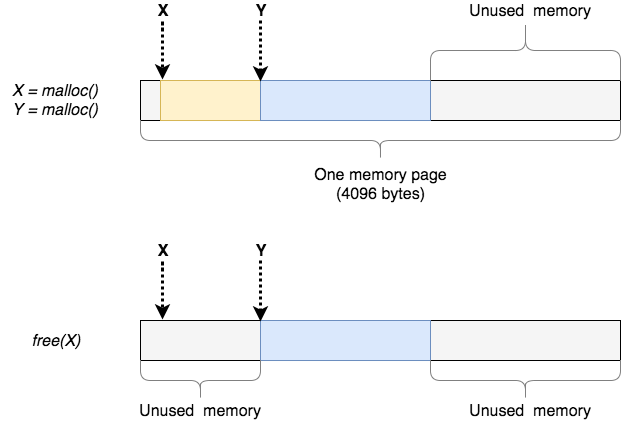
\includegraphics[width=\textwidth]{img/dangling_pointer_basics.png}
    \caption{Memory layout of two small allocations. \emph{X} and \emph{Y} are pointers, referencing their corresponding memory regions. \emph{X} becomes dangling}
    \label{fig:mem_two_small_allocs}
\end{figure}

If a page is known to be unused by the hardware and kernel, then accessing it will trigger a page fault in the kernel, which will generally terminate the application, leading to the best-case scenario described earlier. This is a far more manageable problem than the alternative, because the error is clear, even if in practice it's often difficult to discover the underlying reason, given that time may have passed between the deallocation and attempted access, and so the code executing at the time of access may not have any relation to the code that was responsible for the deallocation. Furthermore, this scenario doesn't generally pose a security problem, as a crashed application is difficult to exploit. Therefore, I will generally ignore this scenario for the remainder of this thesis.

The effect of an unchecked access through a dangling pointer depends on whether or not the referenced memory region has been reused since the time of deallocation. If it hasn't, the data read often will still be valid, and execution may continue without anyone the wiser, masking the bug until a modification in the code or one of the libraries leads to a change in the memory allocation pattern. Otherwise, the data read or overwritten will almost always be a source of unexpected behaviour. One typical case is \emph{type confusion}: the value read or written will be treated as a different type than the value stored there. A string value can be for instance accessed as an integer, causing the characters that make up the string to be interpreted as bytes in an integer, essentially leading to the same behaviour as this code snippet:

\begin{lstlisting}
char *s = "foobar";
int i = *(int *)s;
\end{lstlisting}

This code compiles and runs successfully. What will be the value of \lstinline!i!? Of course, we are deep into undefined behaviour territory here, meaning that the programming language promises nothing. In practice, on x86-64 architectures where the \lstinline!int! C type is 4 bytes long (\lstinline!sizeof(int) == 4!), the result will typically be \texttt{1651470182}, or \texttt{0x626f6f66} in hexadecimal. This makes sense: the string \lstinline!"foobar"! (including the null terminator) is represented by the byte sequence \texttt{0x66 0x6f 0x6f 0x62 0x61 0x72 0x00}. Interpreting it as an \lstinline!int! means reading the first 4 bytes (\texttt{0x66 0x6f 0x6f 0x62}) and assembling it into a multi-byte integer according to the endianness of the processor. My laptop has an Intel CPU in it, which is little endian, meaning that the bytes of an integral type are stored as least significant byte first (this is \texttt{0x62}), followed by bytes of increasing significance; simply put, bytes are interpreted in "reverse order".

Of course, type confusion doesn't have to occur in order for invalid behaviour to occur. For instance, overwriting an Unix file descriptor with the number of characters in a text will typically result in an invalid file descriptor; or consider a buffer's length overwritten by the age of the user; or an integer representing the next free index in an array overwritten by the length of a file in bytes. Once memory corruption occurs, sanity flees.

\section{Overview}

\todo{Better title?}
Dangless is a drop-in replacement memory allocator that provides a custom implementation of the standard C memory management functions \lstinline!malloc()!, \lstinline!calloc()!, \lstinline!realloc()!, \lstinline!free()! and a few others. It aims to solve the problems that dangling pointers lead to by guaranteeing that any access through a dangling pointer will fail, and the application will terminate. It relies on the underlying memory allocator to perform the actual allocation and deallocation. In principle, because Dangless makes no assumptions on the nature or behaviour of the underlying allocator -- referred to as "system allocator" by Dangless --, it should be usable on top of even non-standard implementations such as Google tcmalloc.

Catching dangling pointer accesses is ensured by \emph{permanently} marking memory regions as no longer in use upon deallocation (e.g. a call to \lstinline!free()!). Therefore, during the lifetime of the application, in principle, no other memory will be allocated in such a way that it would visibly alias a previously used location. Of course, the physical memory available is very limited even on modern systems, and not re-using is hopeless. The trick then, is to leave the management of physical memory to the system allocator, and change how the physical allocations are mapped to virtual memory: the address space that user applications interact with. Virtual memory is plentiful: on the x86-64 architecture, pointers are 64-bit long, which in theory means $2^{64}$ bytes of addressable memory. In practice however, on all current processors that use this architecture, only 48 bits are used, which limits the size of the address space we can work with to $2^{48}$ bytes, or 256 terrabytes. That's also not unlimited, but as it turns out, in practice it almost is.

Normally, the difference between physical and virtual memory is entirely hidden from the user code, and is dealt with only by the operating system kernel. This allows the overwhelming majority of users and developers - even programmers working with lower-level languages such as C++ - to work and develop software without ever being aware of the difference, while enjoying the benefits of it. The Linux kernel does provide some system calls that allow the virtual memory to be manipulated, notably \lstinline!mprotect()! which is used to manage access permissions (readable, writeable, executable) of memory regions. This is useful for example when developing just-in-time (JIT) compilers such as the ones employed by browsers to run JavaScript code. Another example is \lstinline!mremap()!, which allows a memory region to be moved almost for free, an ability that makes it useful for garbage collectors for instance. Of course,  \lstinline!mmap()! and \lstinline!munmap()! also primarily work by manipulating virtual memory mappings.

These system calls are sufficient to implement the functionality of Dangless, with some caveats -- in fact, this is exactly how Oscar operates \todo{reference}. The biggest issue is that of performance: system calls are expensive compared to normal memory allocations, and in this scheme, for every single memory allocation, at least one extra system call would be required. The costs and possibilities for optimizations are explored in depth by the Oscar paper.

The solution Dangless uses is a technology called Dune \todo{reference}: a Linux kernel module and library that provides a lightweight virtualization layer based on Intel VT-x. Using Dune, a normal Linux application can choose to enter a virtualized environment where it has ring-0 privileges, allowing it to efficiently and directly manipulate virtual memory mappings and the interrupt descriptor table, while retaining the ability to perform system calls on the host kernel using the \lstinline!vmcall! instruction. In principle, an application running in Dune mode has the best of both worlds; normal Linux libraries and executables are able to run in Dune mode without any modifications, while gaining access to ring-0 features when beneficial. While there is an overhead associated with running in a virtualized environment, especially when performing \lstinline!vmcall!s, in practice this turns out to be negligible for most applications.
